Using the LEV tracking and quantification algorithm mentioned in \ref{sec:LEV}, a quantitative comparison of the LEV is presented in this section. 
Recall that only results from meshes with the 2nd highest spanwise resolution are considered here for brevity, since it was previously established that results between highest and second highest spanwise resolution compare well with each other. Also note that that phase-averaged and spanwise averaged data over multiple cycles is used here.

Figure \ref{fig:zonal_LEV_location} shows the location of the center of the LEV core for different phases after it is ejected from the airfoil surface. 
It is observed that LEV formation for M0 mesh occurs closer to the geometric leading edge, as well as closer to the airfoil surface as compared to the other meshes. 
LEV paths start to converge as the mesh resolution is increased, with Mza2 and Mza3 meshes showing a similar LEV path.


\begin{figure}[H]
	\centering
	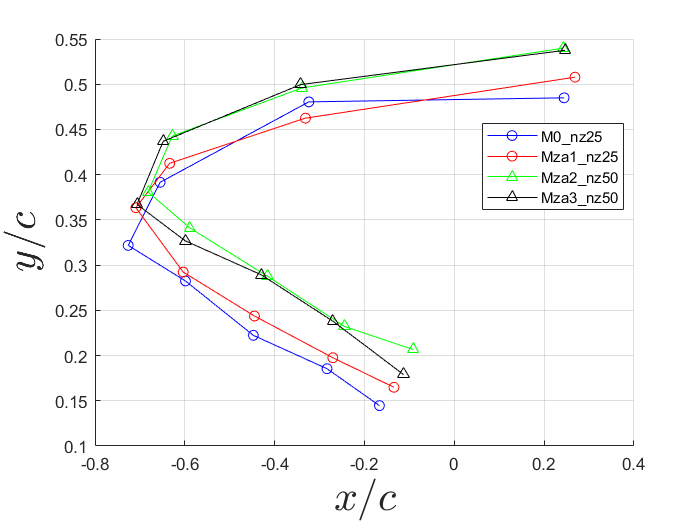
\includegraphics[width=0.75\textwidth]{figures/zonal_adapt_results/LEV/LEV_location}
	\caption{ LEV location for different meshes}
	\label{fig:zonal_LEV_location}
\end{figure}

Figure \ref{fig:zonal_utheta_plots_LEV} shows the tangential velocity profiles for the LEV core for different meshes at phases  $\psi = 240^\circ$,  $\psi = 270^\circ$, and  $\psi = 300^\circ$. 
Note that tangential velocity is computed along multiple radial lines passing through the LEV center, and the mean tangential velocity over these radial lines is shown in \ref{fig:zonal_utheta_plots_LEV}, along with a 95\% confidence interval around the mean. 
The distance from the center of the LEV, $r$, is normalized by the peak radius of the LEV core $r_p$ of the finest mesh Mza3 at that particular phase. 
Here, the peak radius is the radius/location at which maximum tangential velocity is achieved. 
Also note that the maximum of the mean of the tangential velocity is used here. 

For $\psi = 240^\circ$, max $u_\theta$ is achieved around $r/r_p= 0.6$ for M0 mesh and around $r/r_p= 0.8$ for Mza1 mesh, indicating that a smaller LEV core is predicted for M0 and Mza1 meshes as compared to the finer meshes. 
For Mza2 and Mza3 meshes, the max $u_\theta$ is achieved at $r/r_p = 1$. Note that since $r$ is normalized with $r_p$ for Mza3 mesh, max $r/r_p$ will always be 1 for Mza3 mesh. 
Mean tangential velocity profile for both Mza2 and Mza3 meshes, along with the 95\% confidence interval agree with each other. Also note that the large thickness of the confidence interval band around the mean, which can attributed to the LEV core being azimuthally asymmetric, since the LEV in this phase is close to the airfoil surface, as can be seen in Figure \ref{fig:vorticity_zonal_240}. 

For $\psi = 270^\circ$, max $u_\theta$ is achieved around $r/r_p= 1$ for all meshes. M0 and Mza1 meshes predict a lower tangential velocity as compared fto Mza2 and Mza3 meshes. Mean tangential velocity profile for Mza2 and Mza3 meshes agree well with each other with some differences. The confidence interval for Mza3 mesh lies within the confidence interval for Mza2 mesh.

At $\psi = 300^\circ$, for Mza2 and Mza3, both the mean and confidence interval for the tangential velocity matches very well, apart for slight differences at higher $r/r_p$ values. Peak $u_\theta$ for both these meshes is around $r/r_p= 1$.  Also note that the thickness/width of the confidence interval has reduced significantly as compared to the previous phases, showing that the LEV core is more azimuthally symmetric at this phase than the previous phases. Mza1 predicts a lower tangential velocity than the finer meshes, with peak $u_\theta$ around $r/r_p= 1.2$. M0 mesh predicts the lowest tangential velocity, and the peak $u_\theta$ not being reached within $r/r_p= 1.25$.

\begin{figure}[H]
	\centering
	\begin{subfigure}[b]{0.475\textwidth}
	\centering
	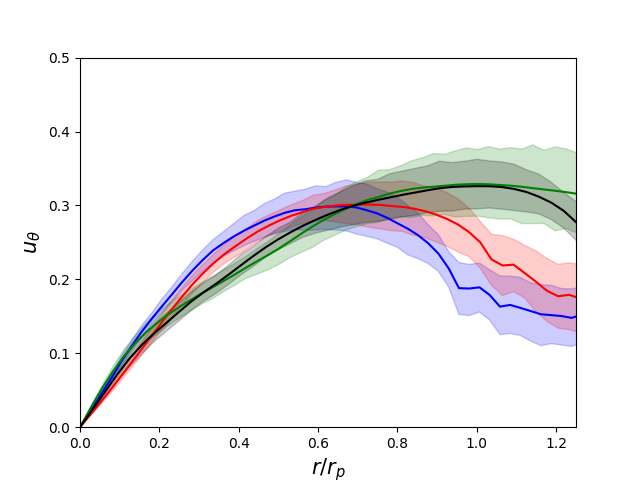
\includegraphics[width=1\textwidth]{figures/zonal_adapt_results/LEV/u_theta/phase_240.png}
	\caption{ $u_\theta$ at $\psi$ = $240^\circ$}
	\label{fig:zonal_utheta_240}
	\end{subfigure}
	\begin{subfigure}[b]{0.475\textwidth}
	\centering
	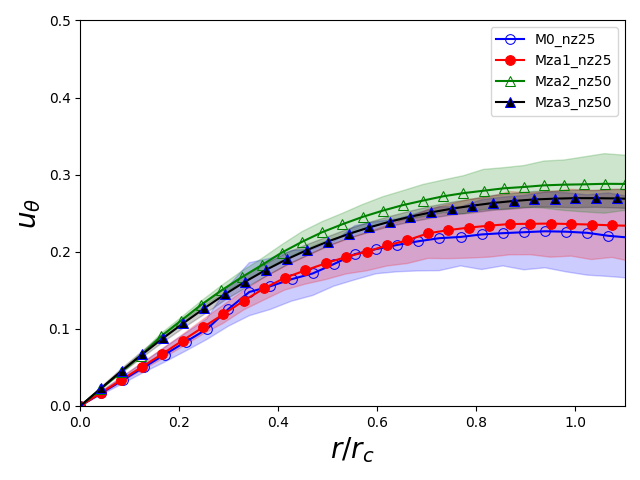
\includegraphics[width=1\textwidth]{figures/zonal_adapt_results/LEV/u_theta/phase_270.png}
	\caption{ $u_\theta$ at $\psi$ = $270^\circ$}
	\label{fig:zonal_utheta_270}
    \end{subfigure}
	\begin{subfigure}[b]{0.475\textwidth}
	\centering
	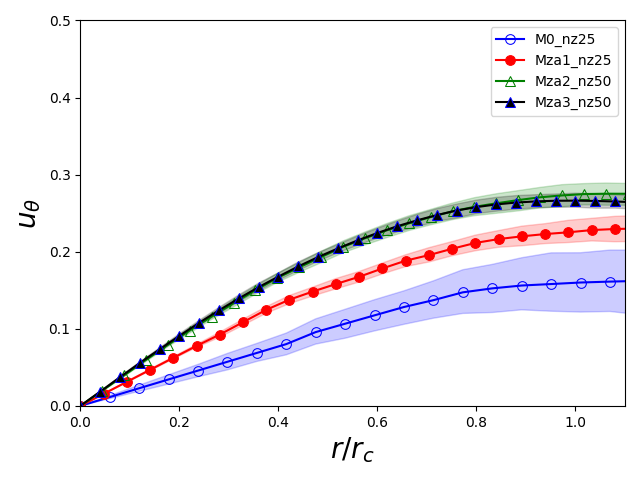
\includegraphics[width=1\textwidth]{figures/zonal_adapt_results/LEV/u_theta/phase_300.png}
	\caption{ $u_\theta$ at $\psi$ = $300^\circ$}
	\label{fig:zonal_utheta_300}
	\end{subfigure}
    \label{fig:zonal_utheta_plots_LEV}
   	\caption{ Tangential velocity profiles of LEV at different phases with 95\% confidence interval}
\end{figure}


Figure \ref{fig:zonal_LEV_radius} shows the radius of the LEV at the peak tangential velocity. 
Recall that tangential velocity is computed along multiple radial lines, and the peak tangential velocity is obtained from this averaged tangential velocity along multiple radial lines. 
In the initial phases when LEV is close to the airfoil surface, Mza2 and Mza3 predict a larger LEV radius than the coarser meshes. 
This difference in size can also be seen in the spanwise vorticity plots shown in Figure \ref{fig:vorticity_zonal_240}.
From phase $\psi = 270^\circ$ and onwards when the LEV is away from the airfoil surface, Mza3 which is the finest mesh, predicts the smallest LEV radius, followed by the second finest mesh, Mza2. 
This is expected, since a finer mesh will have a less diffused vortex core. Also note that M0 mesh completely fails to predict the trend in LEV radius that Mza1, Mza2, and Mza3 meshes show, since the mesh resolution for M0 mesh is poor in the region where LEV traverses through in the later phases.


\begin{figure}[H]
	\centering
	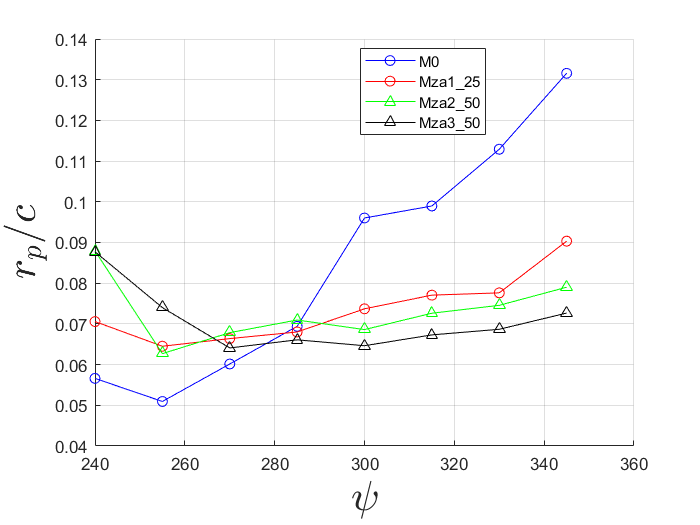
\includegraphics[width=0.75\textwidth]{figures/zonal_adapt_results/LEV/LEV_radius_vp}
	\caption{ LEV radius for different meshes}
	\label{fig:zonal_LEV_radius}
\end{figure}



\begin{figure}[H]
	\centering
	\begin{subfigure}[b]{0.475\textwidth}
		\centering
		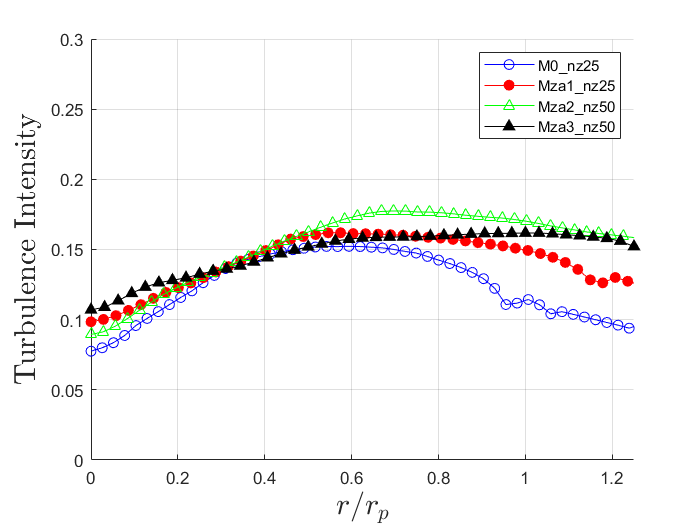
\includegraphics[width=1\textwidth]{figures/zonal_adapt_results/LEV/u_theta/TI_phase_240.png}
		\caption{$\psi$ = $240^\circ$}
		\label{fig:zonal_TI_240}
	\end{subfigure}
	\begin{subfigure}[b]{0.475\textwidth}
		\centering
		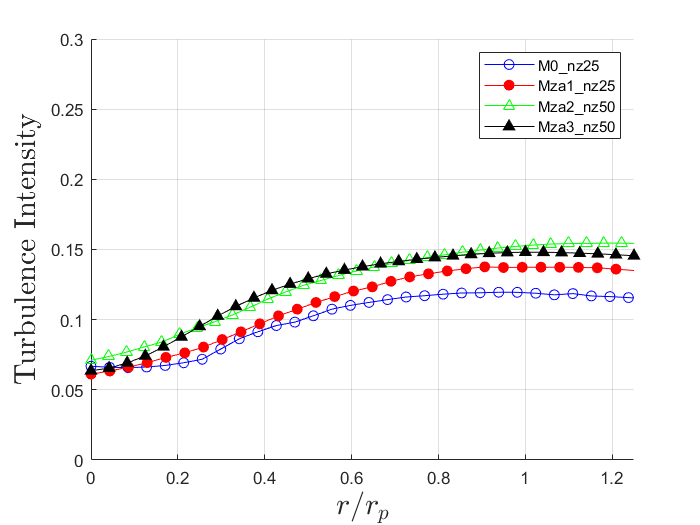
\includegraphics[width=1\textwidth]{figures/zonal_adapt_results/LEV/u_theta/TI_phase_270.png}
		\caption{$u_\theta$ at $\psi$ = $270^\circ$}
		\label{fig:zonal_TI_270}
	\end{subfigure}
	\begin{subfigure}[b]{0.475\textwidth}
		\centering
		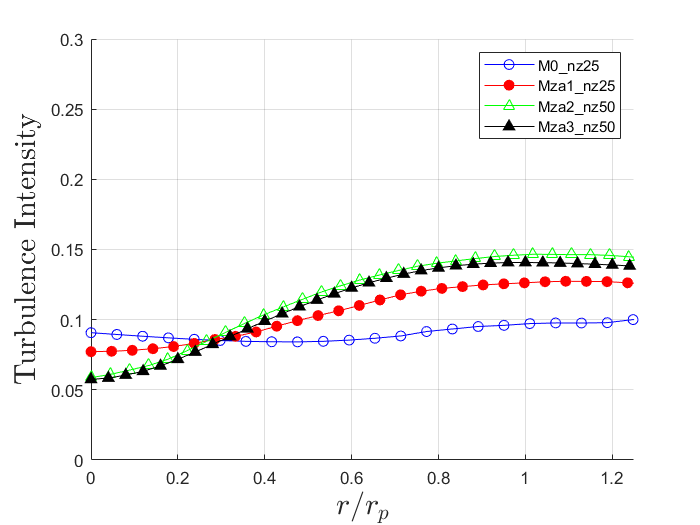
\includegraphics[width=1\textwidth]{figures/zonal_adapt_results/LEV/u_theta/TI_phase_300.png}
		\caption{$u_\theta$ at $\psi$ = $300^\circ$}
		\label{fig:zonal_TI_300}
	\end{subfigure}
	\label{fig:zonal_TI_plots_LEV}
	\caption{ Turbulence Intensity of LEV at different phases}
\end{figure}

